% Chapter Template

\chapter{Results} % Main chapter title

\label{chap:results} % Change X to a consecutive number; for referencing this chapter elsewhere, use \ref{ChapterX}
The solar wind speed data is taken from the instrument Ulysses SWOOPS (todo: Quelle)\\
$v_{sw}$ is assumed to stream only radial for this work.\\
\textbf{Steps vsw} \\ \\

\begin{itemize}
	\item Betrag im SW frame
	\item Winkel im w-space (SW frame)
\end{itemize}

%B-Feld. Von welchem Instrument? auch RTN-System. Genauso Winkel berechnet.
%1-min-Mittel (Gyroradius Zeit zeigen) und entsprechend EpQ-Steps den PHAs zugeordnet.
\clearpage
%
%
%
Todo:\\
Schreiben, dass die velocity Akzeptanzpunkte mit den anteilmäßigen Counts histogrammiert werden? Vielleicht auch ins Data-Kapitel, weil das mit der Normierung gemacht wird...? Sind die Counts überhaupt durch n geteilt?
\\ \\
Here we present the results of the procedure described in chapter \ref{chapter:data}. For creating HE+ VDs from He+ SWICS PHA data we synchronize the selected data (s. \ref{chapter:instrumentation} (triple coincidences) with the SC AA, eigen-velocity and solar wind speed.
This gives us directionally resolved counts from the observed phase space volume.
\\
An example for todo days bla is shown in fig. \ref{fig:counts_50}. Here we histogrammed the counts by utilizing cartesian $w_R$, $w_T$ and $w_N$ bins in solar wind frame. Shown are counts in the $w_T - w_N$ plane from a ``slice'' that has been cut out in $w_R$ direction. The orientation of such a cut is sketched in fig. \ref{fig:sketch_slice_R}. In fig. \ref{fig:counts_50} counts within the range $0.3 <= w_R < 0.5$ have been summarized for each $w_T - w_N$ bin.

(D.h. bei vsw ...)



Dividing the counts by the integrated phase space volume for the observed time, which is binned in the same way and shown in fig. \ref{fig:norm_50}, gives the resulting phase space density, s. fig. \ref{fig:psd_50}.

When Comparing the three figures one can see a change in shape between PSV and PSD bzw. Counts. The PSD doesnt cover als of the scanned PSV and is still a round shape but not as symmetrical as the PSV: We didnt observe HE+ PUIs over all the observed psv but only a distinct central volume.


(In fact a sphere! Nicht darstellbar, deshalb scheibchenweise of width $\Delta w = 0.2$  im Anhang. Man sieht hier außerdem coverage...)


2. peak (not central) in Counts and Norm because of AA: where did we look most... vanishes by normalization... no physics but an artificial effect of the measurement

3. psd: majority streams central in this example

4. (?) ring in norm due to psv auf anderen Schalen; da größere Volumina wegen v





noch einen anderen Fall zeigen: anderer Zeitraum, anderes Ergebnis:
Hier sorgt die Normalisierung dafür, dass ein angebliches Ringfeature verschwindet. Auch hier majority radial.

-- andere Schnitte
außerdem noch T und N Schnitt möglich


Ergebnis kann man in noch in anderen Pr. zeigen:
andere Projektionen:
--- Skymap

--- 1D






\clearpage
\subsection{Slices}


%%% R %%%

\begin{figure}[h]
	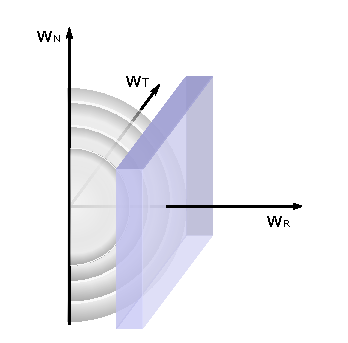
\includegraphics[width=.4\textwidth]{Figures/slice_R2.pdf}
	\centering
	\caption{todo}
	\label{fig:sketch_slice_R}
\end{figure}

\begin{figure}[h]
	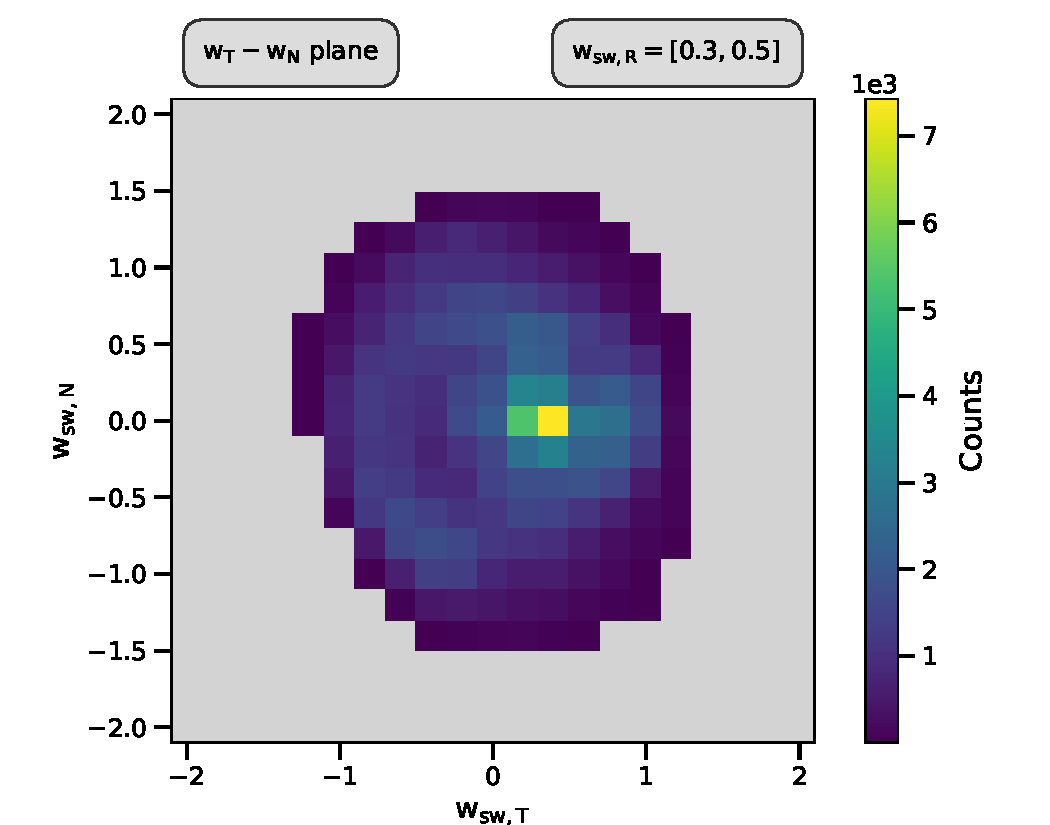
\includegraphics[width=.8\textwidth]{Figures/cart_50_counts_R.pdf}
	\centering
	\caption{todo}
	\label{fig:counts_50}
\end{figure}

\begin{figure}[h]
	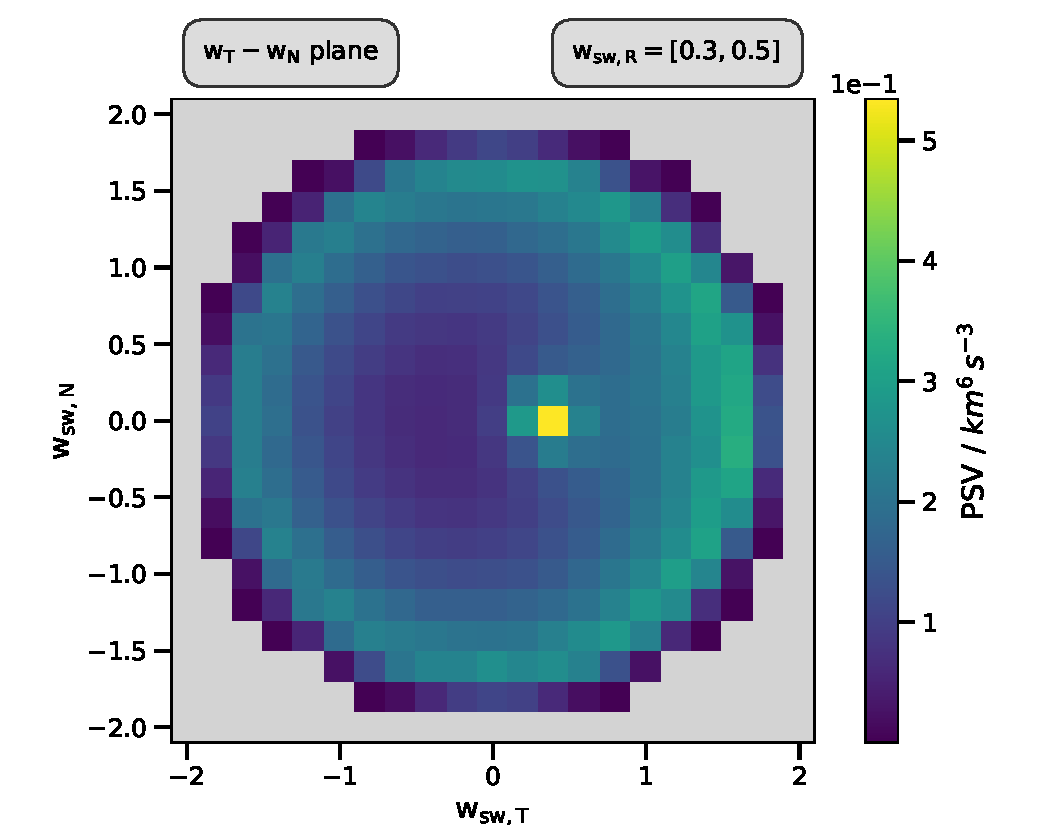
\includegraphics[width=.8\textwidth]{Figures/cart_50_norm_R.pdf}
	\centering
	\caption{todo}
	\label{fig:norm_50}
\end{figure}

\begin{figure}[h]
	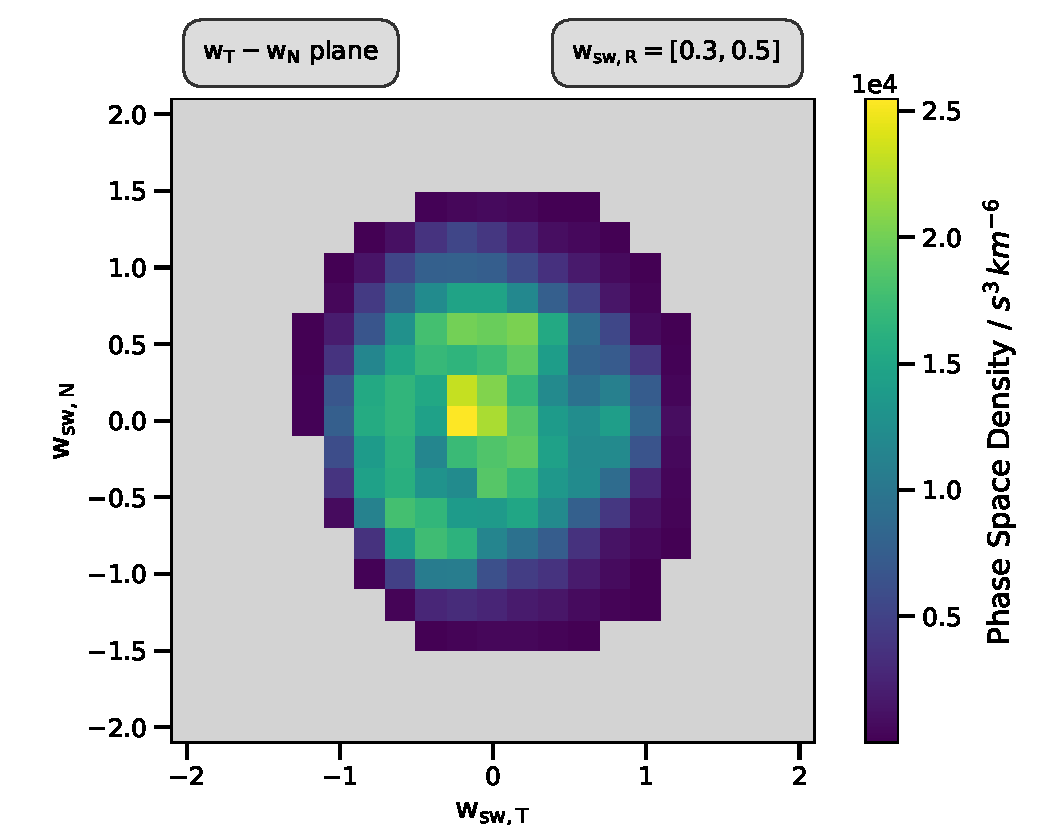
\includegraphics[width=.8\textwidth]{Figures/cart_50_ps_R.pdf}
	\centering
	\caption{todo}
	\label{fig:psd_50}
\end{figure}

\begin{figure}
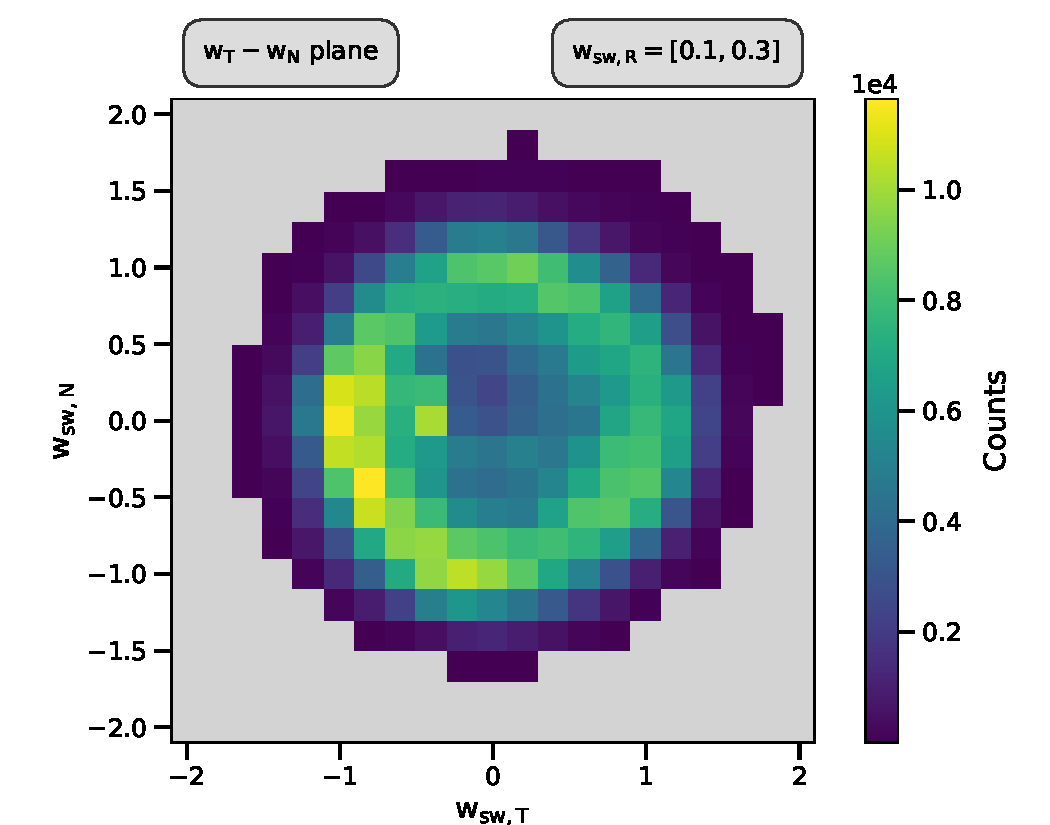
\includegraphics[scale=.28]{Figures/cart_lang_R_counts.pdf}
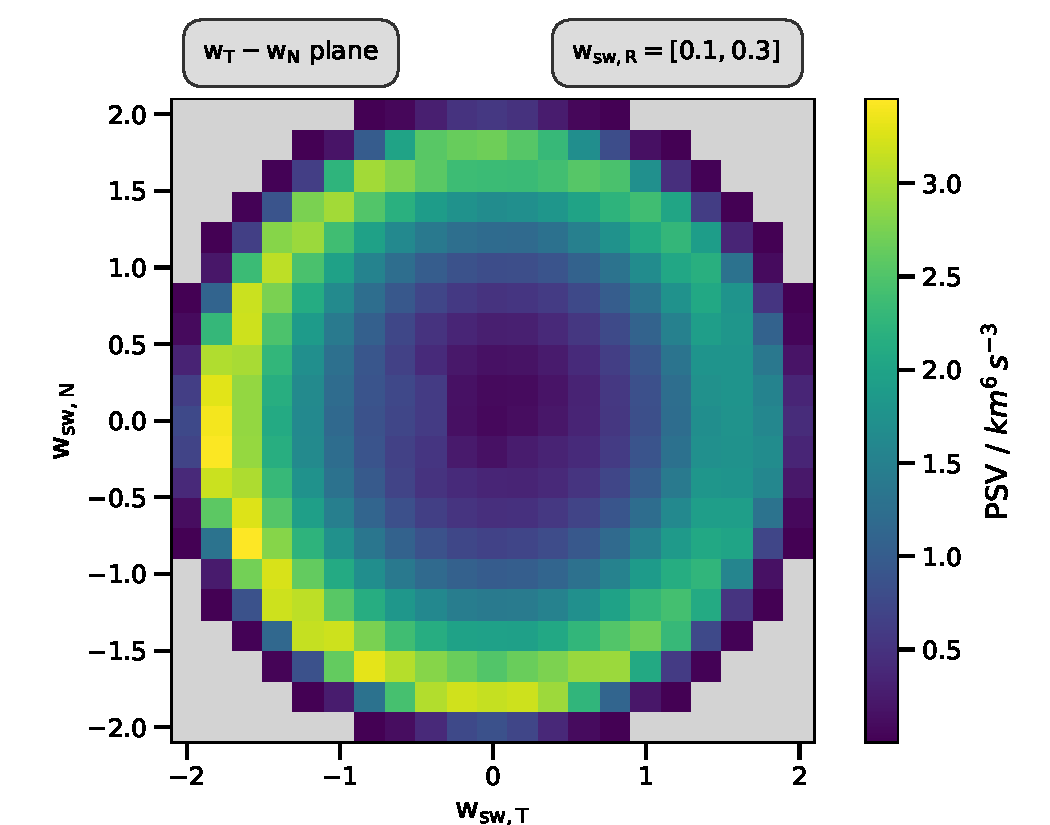
\includegraphics[scale=.28]{Figures/cart_lang_R_norm.pdf}
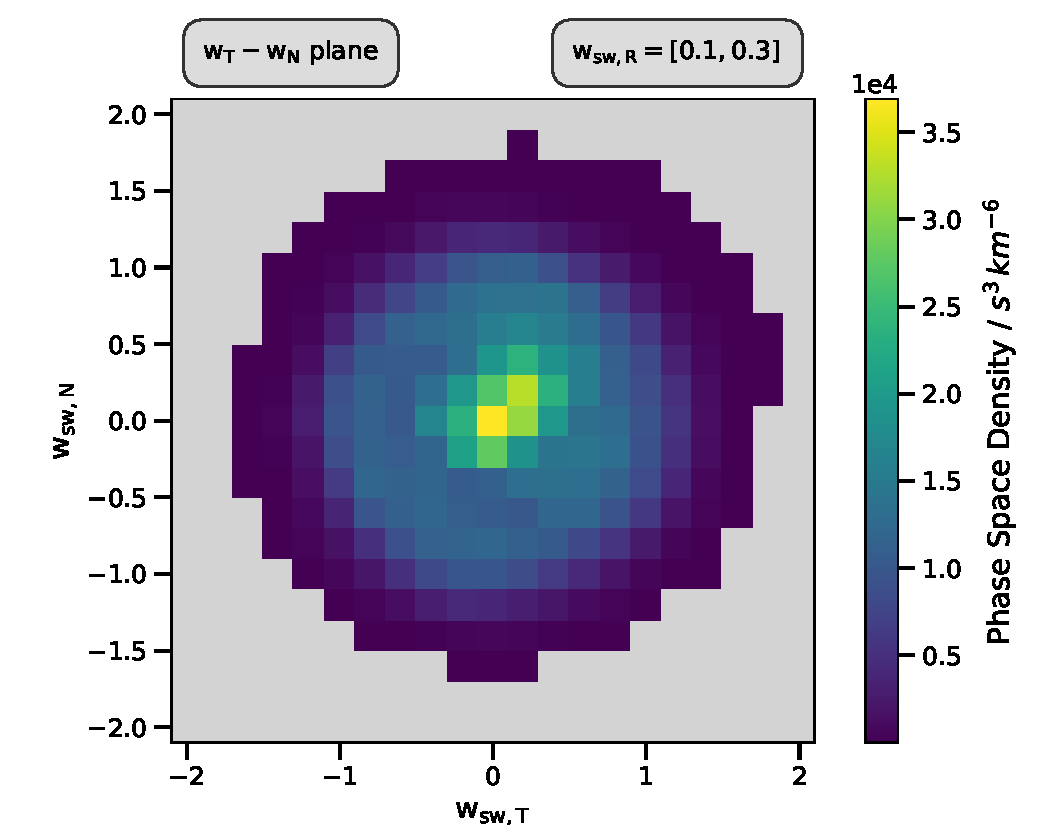
\includegraphics[scale=.4]{Figures/cart_lang_R_psd.pdf}
\end{figure}



%%% T %%%
\begin{figure}[h]
	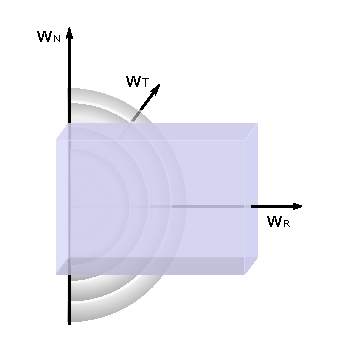
\includegraphics[width=.4\textwidth]{Figures/slice_T2.pdf}
	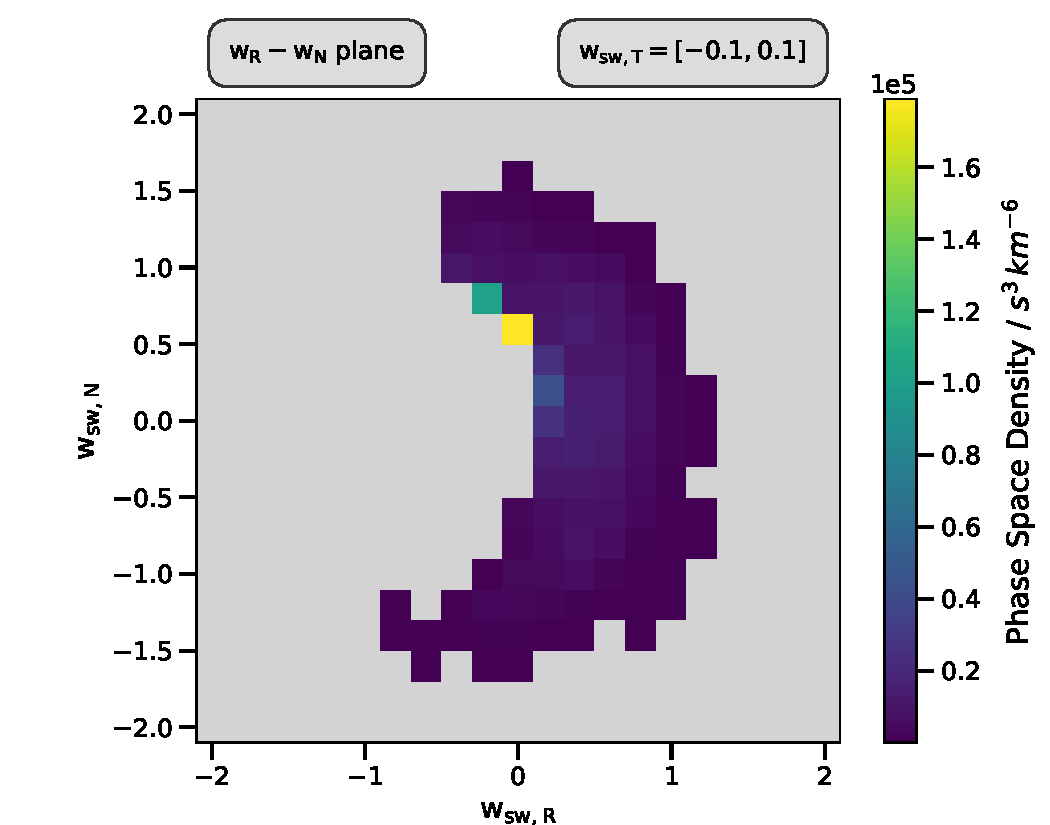
\includegraphics[scale=.45]{Figures/slice_psd_T.pdf}
	\centering
	\caption{todo}
	\label{fig:sketch_slice_T}
\end{figure}

%%% N %%%

\begin{figure}[h]
	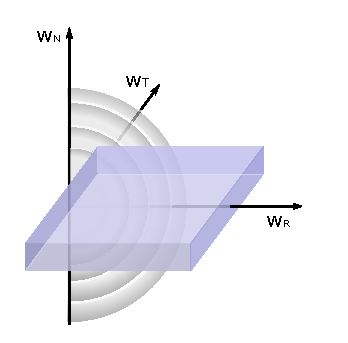
\includegraphics[width=.4\textwidth]{Figures/slice_N2.pdf}
	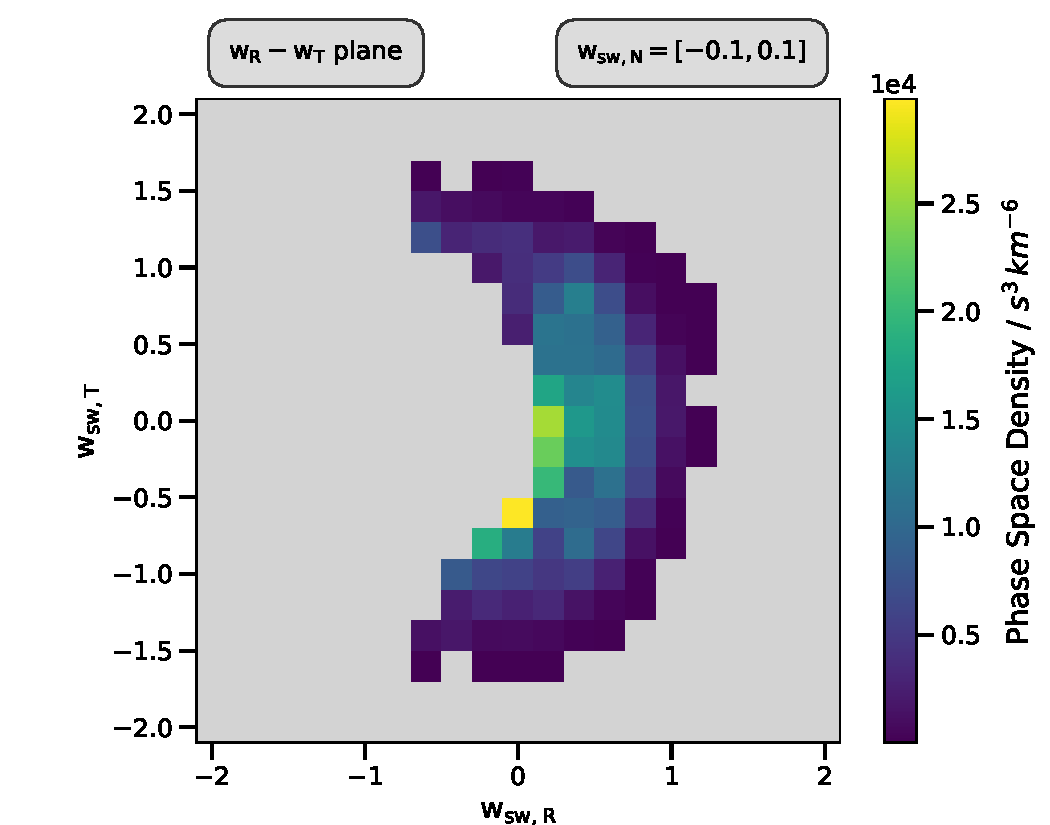
\includegraphics[scale=.45]{Figures/slice_psd_N.pdf}
	\centering
	\caption{todo}
	\label{fig:sketch_slice_N}
\end{figure}


%
%
%
\clearpage
\subsection{Skymaps}
\begin{figure}[h]
	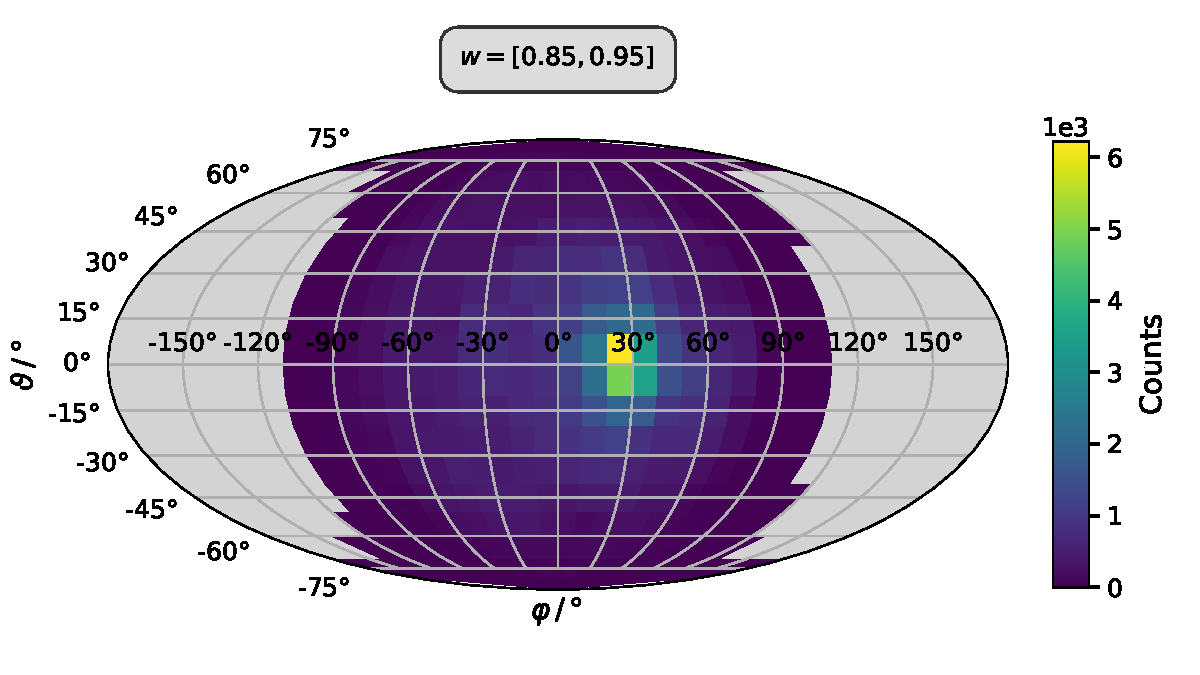
\includegraphics[width=1\textwidth]{Figures/sky_counts.pdf}
	\centering
	\caption{todo}
	\label{fig:todo}
\end{figure}
\begin{figure}[h]
	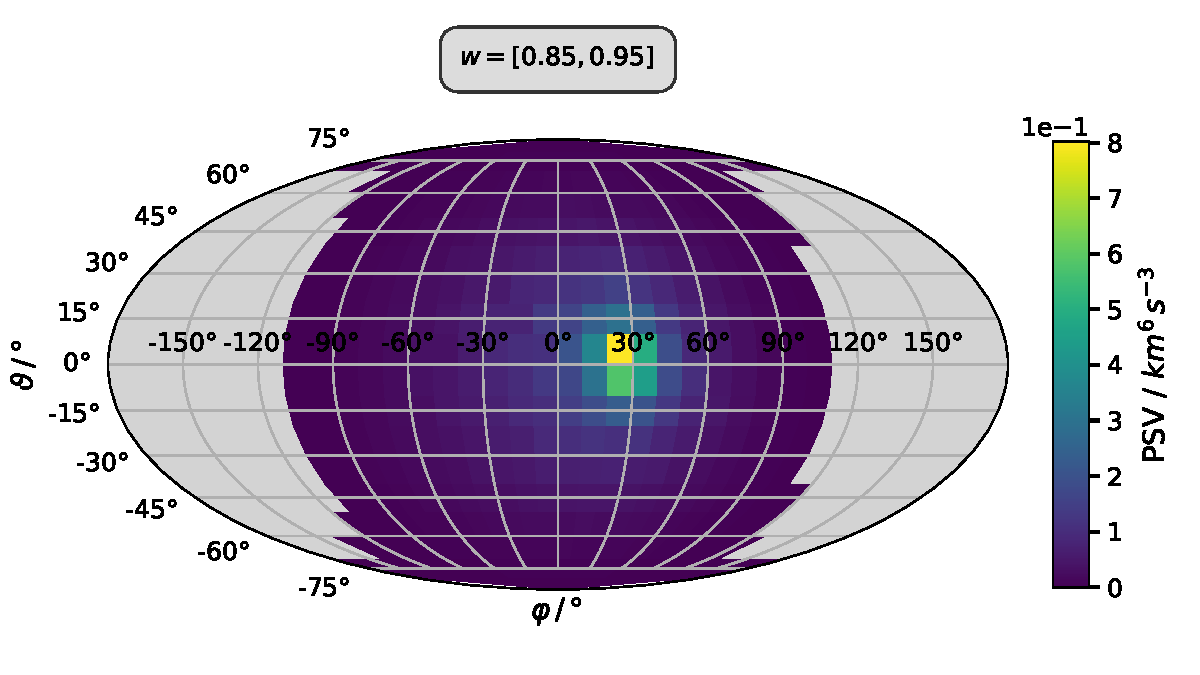
\includegraphics[width=1\textwidth]{Figures/sky_norm.pdf}
	\centering
	\caption{todo}
	\label{fig:todo}
\end{figure}
\begin{figure}[h]
	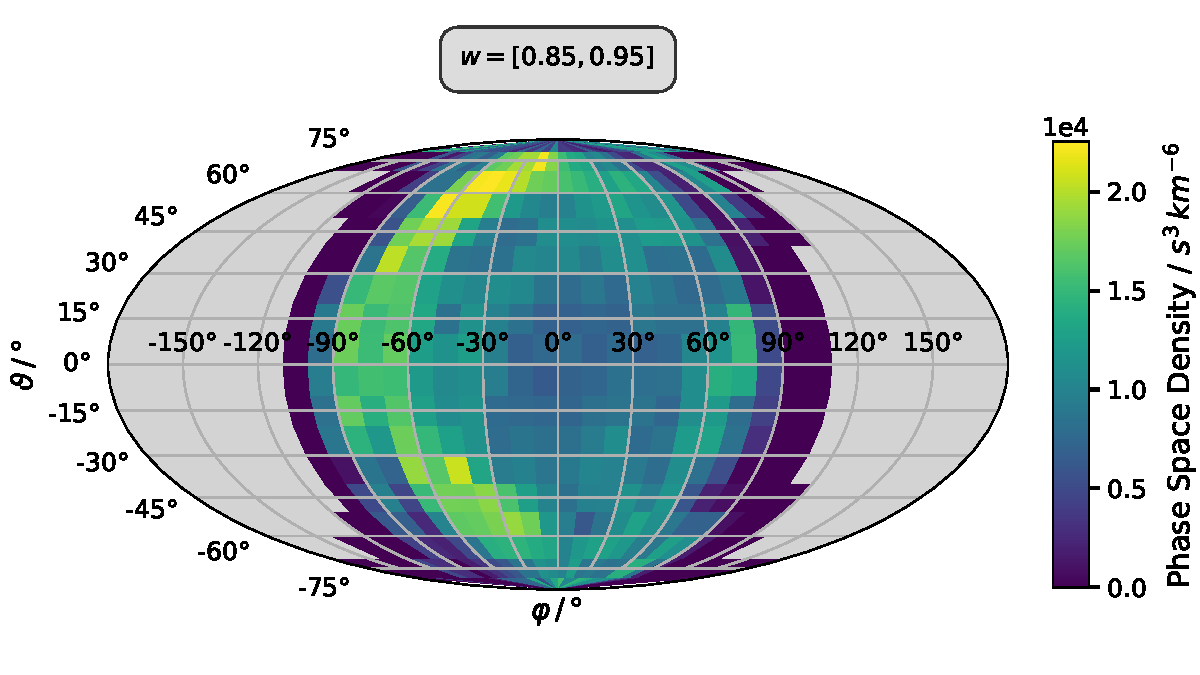
\includegraphics[width=1\textwidth]{Figures/sky_ps.pdf}
	\centering
	\caption{todo}
	\label{fig:todo}
\end{figure}
%
%
%
\clearpage
\subsection{1D}

\begin{figure}[h]
	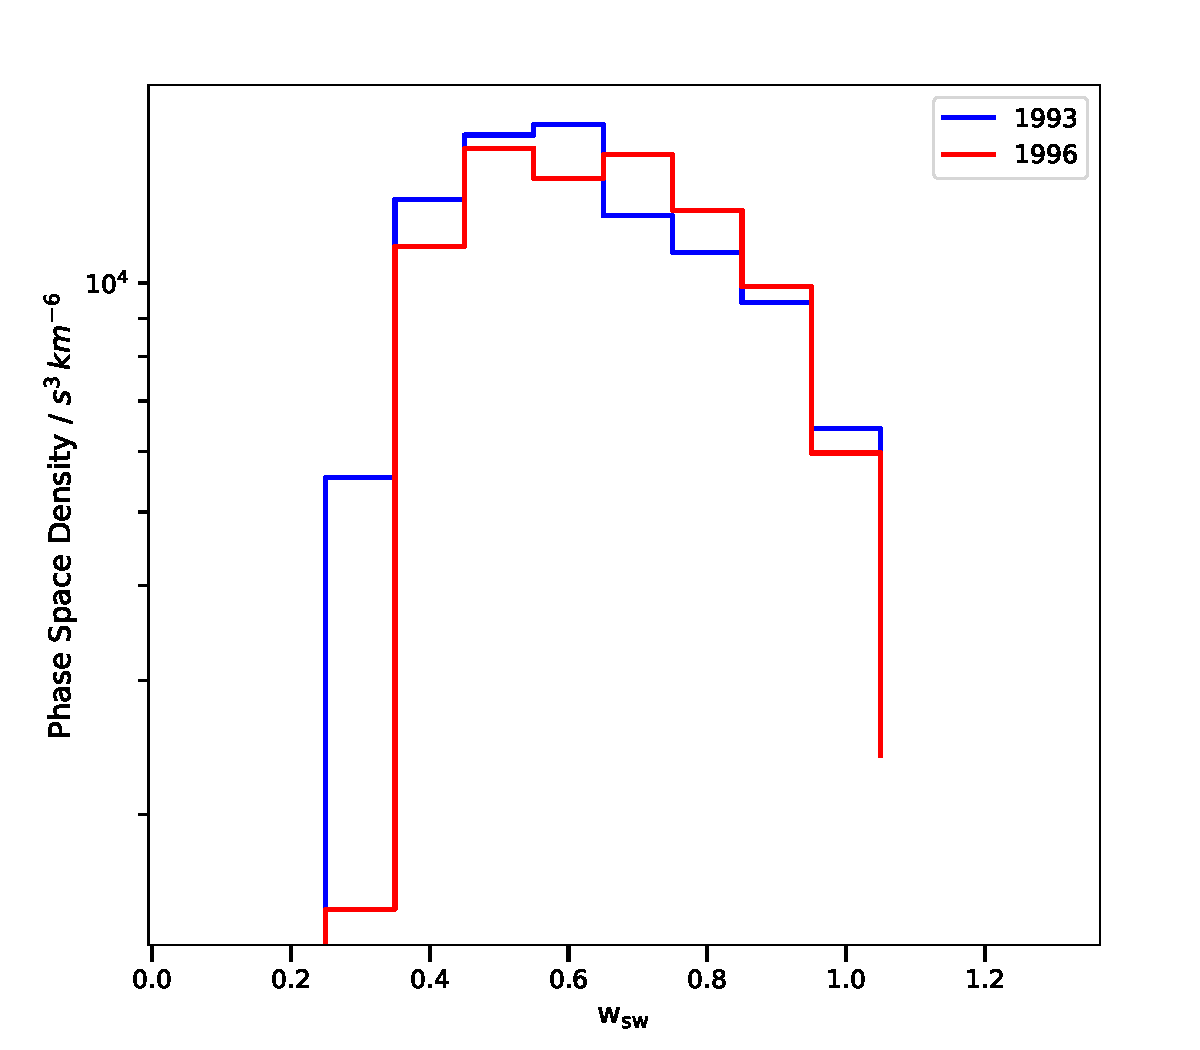
\includegraphics[width=.8\textwidth]{Figures/1D.pdf}
	\centering
	\caption{todo}
	\label{fig:todo}
\end{figure}
%
%
%
\clearpage
\section{Loose Ends}
\begin{itemize}
	\item andere Daten: B, vsw (Swoops: als vsw wird Protonengeschw. genommen. Ist das überhaupt richtig, ist das der Referenzframe? Und Annahme, dass vsw rein radial ist)
	\item Die Sache mit dem BRW ab 2003
	\item Englisch: Relativpronomen, Kommasetzung, British/American
	\item $\mathrm{He^{+}}$ einheitlich, mathrm
	\item Tempus?
	\item kursiv / nicht kursiv wie war das nochmal
	\item spinrate drin?
\end{itemize}
